\chapter{Classifying Transformation Networks
    \pgsize{15 p.}
}
\label{chap:classification}

\mnote{Quality property dimensions}
In the previous chapters, we have discussed how correctness of transformation networks can be achieved under the assumption of independent development and modular reuse of the individual transformations.
Artifacts of the software development process, and thus also transformation networks, have, however, further relevant properties than functional correctness.
Other properties especially concern the quality of artifacts regarding several dimensions, as also defined by ISO standard 25010~\cite{iso25010}.
For the operation of a piece of software, besides functionality also its performance, usability, reliability, and security are relevant, whereas for its development especially its maintainability and portability are of interest~\cite[Tab.~2]{iso25010}.

\mnote{Focus on maintainability}
These dimensions of quality properties are directly related to the stakeholders for which they are relevant.
While most property dimensions are related to the operation of a system, which in our case is the transformation network, and are thus relevant for users, i.e., for the people developing a system whose artifacts are kept consistent with transformations (see \autoref{chap:networks:specification_process}), especially maintainability is important for those who develop and maintain a transformation network~\cite[Tab.~2]{iso25010}.
Although all these properties are relevant and have to be considered when developing transformation networks, we explicitly put the focus on those that are relevant for developers of transformations and transformation networks (see \autoref{chap:introduction:objective:benefits}).
Thus, in the following, we particularly focus on properties regarding \emph{maintainability} of a transformation network in addition to its functionality.

\mnote{Topology effects on properties}
In our motivation in~\autoref{chap:introduction}, we have derived several assumptions regarding the process of transformation network construction.
In particular, we have identified independent development and modular reuse of transformations to be essential assumptions, which directly imply that consistency relations may be defined and preserved transitively and repeatedly across different paths of transformations, thus inducing a dense graph of transformations.
Since different qualities properties highly depend on the topology of a transformation network, we aim to identify these dependencies and thus discuss which topologies of transformation networks should be distinguished, independent from the initial assumptions that we have made.
We then discuss how these topologies influence quality properties and identify trade-offs between these properties, especially concerning functional correctness and reusability.
Instead of assuming modular reuse and then deriving how to achieve functional correctness, as it was the goal of the previous chapters, we consider topologies with inherent correctness properties and investigate how to improve quality properties, such as their independent reuse.

\mnote{Subordinate contributions}
This chapter thus constitutes our contribution \autoref{contrib:quality:topologies}, which consists of two subordinate contributions: a discussion of quality properties and their manifestation in transformation networks; and a classification of transformation network topologies with a discussion about their impact on properties.
It answers the following research question:

\researchquestionrepeat{rq:quality:properties}

\mnote{Benefits of contributions}
With the insights in this chapter, transformation developers and users become aware of further quality properties of transformation networks besides correctness.
They understand how the topology of a network affects these properties and, thus, between which of them trade-off decisions for their improvement have to be made.

\mnote{Publication of contributions}
Parts of the contributions in this chapter have been published in previous work~\owncite{klare2018docsym}.
This especially concerns the identification of general relations between topologies and quality properties of transformation networks as well as the implication of trade-offs between these properties.


\section{Properties of Transformation Networks}
\label{chap:classification:properties}

\mnote{Further functional properties}
The most essential property of transformation networks, which we have also considered in the last chapters, is correctness, or more precisely \emph{functional correctness}, according to ISO standard 25010~\cite[p.~11]{iso25010}.
In addition to its correctness, functionality can be regarded in terms of \emph{completeness} and \emph{appropriateness}~\cite[p.~11]{iso25010}.
While completeness concerns the degree to which functions cover all intended objectives, appropriateness is the degree to which functions facilitate the conduction of tasks to achieve the intended objectives.
In terms of a transformation network, completeness represents whether the network is able to preserve all consistency relations, which requires transformations for all existing relations to keep consistent to be defined.
Since appropriateness especially concerns manual effort, it is not as relevant in a fully automated process. Appropriateness would especially be of interest if the user is involved in the consistency preservation process by clarifying its intent or making necessary decisions to adapt models for being consistent, which can influence how far the automation facilitates the process of consistency preservation.
Thus, in addition to functional correctness we also discuss functional completeness as a relevant property and relate it to our requirement of \emph{universality}, defined in \autoref{chap:introduction}.

\mnote{Quality properties regarding maintainability}
In our work, we focus on properties of transformation networks that are relevant for their developers (see \autoref{chap:introduction:objective:benefits}).
Thus, in addition to functional properties of such networks, we especially consider properties regarding their \emph{maintainability}~\cite[Tab.~2]{iso25010}, which describe the \enquote{degree of effectiveness and efficiency with which a product or system can be modified by the intended maintainers}~\cite[p.~14]{iso25010}.
Maintainability includes the properties \emph{modularity}, \emph{reusability}, \emph{analyzability}, \emph{modifiability}, and \emph{testability}~\cite[pp.~14]{iso25010}.
We have already covered the former two properties of modularity and reusability implicitly in our assumption of \emph{modular reuse}, as well as analyzability in the goal of \emph{comprehensibility}.
In previous work~\owncite{klare2018docsym}, we also discussed properties of transformation networks but without basing them on a common understanding defined by the mentioned ISO standard.


\subsection{Correctness}

\mnote{Central importance of correctness}
According to ISO standard 25010~\cite{iso25010}, functional correctness denotes to which degree a system, in our case a transformation network, provides correct results.
We have intensively discussed this property in the previous chapters, starting with a definition of \emph{correct results} in \autoref{chap:correctness} and discussing how to achieve transformation networks that fulfill such a correctness notion in \autoref{chap:compatibility} to \autoref{chap:orchestration}.
We do thus not discuss that property again, but emphasize its central importance for a transformation network to be useful, as an incorrect transformation network leading to models of a system description that are inconsistent %, in the worst case without informing the developer about it, 
will hardly provide relevant benefits.


\subsection{Completeness}

\mnote{Universality}
According to ISO standard 25010~\cite{iso25010}, functional completeness describes to which degree provided functions cover all objectives.
Applied to transformation networks, this means to which degree such a network can preserve consistency according to consistency relations, be they explicitly defined or only intended by a transformation developer.
Completeness of the individual transformations as well as of the transformations are both covered by their notions of correctness (see \autoref{def:synchronizingtransformationcorrectness} and \autoref{def:transformationnetworkcorrectness}).
It does, however, assume an even broader notion of what we introduced as \emph{universality} in \autoref{chap:introduction}.
While we have introduced universality as the ability to process transformation networks of arbitrary topology, an even broader notion would require the applicability of transformation network to every project in which artifacts need to be kept consistent.
Thus, it would first require that the artifacts to keep consistent are represented in a form that is required to define transformations between them.
More precisely, the artifacts to keep consistent need to conform to some kind of modeling formalism, such as the one we proposed in \autoref{chap:networks:models} based on the \gls{EMOF} standard~\cite{mof}.

\mnote{Non-modeled artifacts}
If the artifacts, or more generally the models, to keep consistent are not represented in a format conforming to such a modeling formalism, a metamodel for them needs to be defined and their representation may need to be transformed into an instance of such a metamodel.
This is especially the case for proprietary tools that do not use a common format to represent their artifacts.
For many popular tools, however, metamodels based on \gls{EMOF} or Ecore have already been reverse-engineered, such as 
MATLAB/Simulink~\cite{heinzemann2013Reconfiguration-CBSE,son2012Simulink-CAGGIE,armengaud2011Safety-WCE}.
In addition, the \gls{EMF} as a popular modeling framework provides an importer for XML-based specifications of metamodels~\cite[pp.~86]{steinberg2009emf}.
Tools, especially from engineering domains, often provide XML-based representations of their artifacts, such as the electronic circuit design tool EPLAN~\cite{eplan} or the exchange format for automation system design in AutomationML~\cite{automationML}.
Defining a metamodel for a specific modeling formalism, such as Ecore, and representing artifacts as models of it is always necessary when modeling tools for that formalism shall be applied, for which transformations are only one example.
Frameworks for generating graphical editors or model analyses could be further tools to be applied~\owncite{klare2017models}.
Thus, such an integration of artifacts into model-driven processes is part of separate research.

\mnote{Integration approach}
In our research, we have also developed and proposed such an approach to integrate artifacts into model-driven processes~\owncite{klare2017models, klare2019modelsward}.
It is based on the insight that code often contains models implicitly.
The tools, whose artifacts we want to keep consistent, usually have definitions of metamodels of their artifacts defined within their source code, but only as a simple structure of classes instead of am explicit metamodel according to some modeling formalisms.
For example, Java graph libraries need to contain a metamodel for representing graphs, but this is usually just represented by a set of classes and not an explicit metamodel according to some modeling framework.
This also applies to programming languages, for which parsers contain metamodels for their \gls{AST} representations.
We have proposed an approach that makes these implicit metamodels explicit to apply modeling tools, such as transformations for consistency preservation, to them~\owncite{klare2017models, klare2019modelsward}.
Since that topic and especially the proposed approach is important for applying transformation networks, but also has further, broader application areas, we do not further discuss it in this thesis but refer to our previous work for details about it.


\subsection{Maintainability}

\mnote{Influencing factors}
We have identified maintainability as a dimension of quality properties with central importance for developers of transformations and transformation networks.
According to ISO standard 25010~\cite{iso25010}, maintainability includes modularity, reusability, analyzability, modifiability and testability.
We discuss for these properties how they manifest in transformation networks and especially how they are related to each other.
We do not aim to measure these properties, which is why we do not propose specific metrics for them.
For source code, it has been shown to be hard to assess its quality, e.g., to measure modifiability in terms of a correlation with the number of defects~\cite{Gyimothy2005ValidationMetrics-TSE, Yu2002FaultPrediction-ECSMR}, and that only few metrics provide a correlation to, for example, the number of defects.
In fact, we only aim at identifying the influencing factors for these properties instead of a measure for them anyway, especially with respect to topologies of the transformation network, which we discuss afterwards.

\begin{properdescription}
    \item[Modularity:] 
    Modularity is the degree to which a program, and thus also a transformation network, is composed of components such that changes only influence a part of it~\cite[p.~14]{iso25010}.
    This property degrades when having multiple paths of transformations expressing the same consistency relations, as then these paths depend on each other and may be contradictory. 
    Having such multiple paths can lead to incompatibilities (see \autoref{chap:compatibility}) or situations in which no consistent orchestration of the transformations exists (see \autoref{chap:orchestration}), and thus degrade modularity.
    \item[Reusability:]
    Reusability is the degree to which assets, such as the single transformations of a transformation network, can be used in more than one system~\cite[p.~15]{iso25010}.
    In terms of a transformation network, reusability of a transformation is given if it is independent from the other transformations and can be used together with others in a different context.
    This conforms to our notion of independent development and modular reuse, given as assumptions in \autoref{chap:introduction}.
    Reusability profits from having all relations between the involved metamodels expressed explicitly, i.e., directly between each pair of metamodels and not only transitively across others.
    This leads to multiple expressions of the same relations transitively across different paths of transformations, but allows subsets of the transformations to be used in a different context, in which only a subset of the metamodels is used.
    For example, having the relation between \gls{PCM} and Java expressed directly instead of only expressing it transitively across \gls{UML} enables its reuse in other system development scenarios in which \gls{UML} is not used at all.
    Thus, reusability degrades when modularity improves.
    \item[Analyzability:] 
    Analyzability is the degree to which the impact of a change can be assessed effectively and efficiently or to which defects can be identified afterwards~\cite[p.~15]{iso25010}.
    On the one hand, this is important for the single transformations, as analyzing the impact of a change especially concerns the intended change of the behavior of a transformation. That is, however, also a topic of dedicated research about transformation validation and verification~\cite{cabot2010VerificationInvariants-JSS, rahim2015SurveyTransformationVerification-SoSym, azizi2017ContractVerification-ICCKE, vallecillo2012FormalTesting-FMMDE}.
    On the other hand, this is important for the interplay of transformations, thus how a change to one transformation affects interoperability with the others.
    This is, again, directly related to the existence of multiple paths of transformations preserving consistency to the same relations, as it influences how many other transformations may be affected and potentially need to be updated due to the modification to one of them.
    Consequently, the more relations are preserved across multiple paths of transformations, the more transformations may be affected by a single change and introduce interoperability problems that may be hard to analyze (see \autoref{chap:orchestration}).
    Analyzability is also related to the notion of comprehensibility that we have introduced in \autoref{chap:introduction}. The lower analyzability is, the harder it becomes for a transformation developer to comprehend what the combination of transformations actually does and how an intended change can be performed and what its impact is.
    We have also used comprehensibility to motivate the design of our orchestration algorithm in \autoref{chap:orchestration:algorithm}, which is driven by the goal of easing the analysis of failures of the transformation network, analogous to analyzability.
    Thus, analyzability improves with modularity.
    \item[Modifiability:]
    Modifiability is the degree to which a system can be modified without introducing defects or degrading quality~\cite[p.~15]{iso25010}.
    It is directly influenced by modularity and analyzability, as also stated by the ISO standard~\cite[p.~15]{iso25010}.
    In terms of a transformation network, this can include the adaptation of existing transformations or the extension of an existing network with further metamodels and transformations.
    The same arguments as for modularity and analyzability apply and thus modifiability improves and degrades with modularity of the transformation network.
    For example, the complexity of adding a new transformation, which is covered by modifiability, depends on the number of transformations that already, and in particular transitively, preserve relations between the two metamodels to define the new transformation between.
    \item[Testability:]
    Testability is the degree with which test criteria can be effectively and efficiently established and evaluated by test cases for a product~\cite[p.~15]{iso25010}, such as a transformation network.
    While there are many influencing factors for testability, such as encapsulation and coupling within the implementation, it is, again, also influenced by the number of transformation paths across which consistency relations are preserved.
    The more paths of transformations preserving the same consistency relations exist, the larger is the set of models to be considered and transformations to be executed for testing correctness of preserving consistency according to a certain relation.
    This increases complexity of the tests to perform.
    Testability is also highly related to the notion of comprehensibility that we have introduced in \autoref{chap:introduction} as we have also discussed for analyzability. 
    The higher the number of transformations that need to be executed to detect a failure, the more complex we can expect the process of identifying the causing mistake to be (see \autoref{chap:errors}).
    Testability, just like analyzability and modifiability, thus improves with modularity.
\end{properdescription}

\mnote{Opposed properties}
The discussion shows that the existence of multiple paths of transformations preserving consistency to the same consistency relations reduces modularity, modifiability, analyzability and testability, while improving reusability.
This is due to the fact that multiple representations of the same consistency relations induce dependencies, which reduce modularity, and can contain conflicts, reducing modifiability.
The increased complexity reduces analyzability and testability.
Reusability is, however, improved, because relations are not only represented transitively.
In the following, we identify relevant topologies of transformation networks that reflect the effects on properties of having multiple transformation paths preserving consistency to the same relations, and discuss their impact on properties.

%Modularity is degree to which a program is composed of components such that changes only influence a parts.
%This fits to our needs, because if we have a dense graph, modularity is low, as a change in one transformation may affect several others that need to be changed to restore compatibility and correctness.


% \begin{copiedFrom}{DocSym}

% %Even if independently developed transformations are interoperable, as discussed before, higher-level challenges remain when considering the way in which transformations express relations or occur if compatibility between the transformations is not given.
% %Those challenges cannot be solved simultaneously, but induce trace-off decisions that have to be made regarding the way in which transformations are specified. %, as not all of them can be solved simultaneously.
% %Depending on the topology of transformations that preserve the consistency, those challenges are addressed differently, which will be discussed afterwards. %in the subsequent section.
% %We present already identified challenges in the following. % and discuss them regarding the combination of binary transformations. % as the state-of-the-art for multi-model consistency preservation.

% % \compactsubsection{Uniqueness}
% % Each consistency relation should only have to be specified once to reduce effort and the risk of contradictory specifications.
% % In terms of transformations, this means that there should only be one path in the graph induced by the transformations to propagate information from one model to another.
% % Using existing transformation languages, not knowing which relations have already been realized in which transformations can lead to duplication.
% % This is especially the case, if one transformation is only the subsumption of others, like in \autoref{fig:binary_combination_example}. %of components and classes defined by
% % %mapping \ac{PCM} to \ac{UML} components, \ac{UML} components to \ac{UML} classes, and those classes to Java classes. 
% % \todo{Das folgende ist eigentlich schon im vorigen Abschnitt diskutiert worden}
% % If the relation \ref{fig:Example:R3} between \ac{ADL} and Java is specified additionally to the transitive relation over \ac{UML}, the transformations derived from it must ensure that after creating an \ac{ADL} component only one Java class is created, that all necessary trace links are created, and that additional constraints, such as the convention to append \enquote{Impl} to the name, are consistently defined.

% \begin{properdescription}
% \item[Compatibility:]
% Transformations preserve consistency, but also have to be consistent among themselves, i.e., they have to adhere to the same consistency relations, referred to as \emph{compatibility}.
% %Contradictory specifications can, for example, arise from inconsistent realizations of the same consistency relations.
% If, in our example in \autoref{fig:introduction:scenario_topologies}, the relation %\ref{fig:prologue:binary_combination_example:R3} 
% between \gls{ADL} and Java is realized in addition to the transitive relation %$\mbox{\ref{fig:prologue:binary_combination_example:R1}} \concat \mbox{\ref{fig:prologue:binary_combination_example:R2}}$ 
% over \gls{UML}, both relations must contain the same name attribute mapping.
% If the \gls{ADL} to Java transformation adds an \enquote{Impl} suffix~\cite{langhammer2017a}, whereas the transformations over \gls{UML} omit that, they are \emph{incompatible}.
% This can lead to propagation cycles due to alternating values, and to results depending on the transformation execution order. %depends on the transformation execution order. %, which means that the result depends on the execution order of the transformations. % (e.g., the propagation from \ac{PCM} to Java or from \ac{UML} to Java), the result differs (in the example the name of the class)
% %\end{inparaenum}
% While \emph{compatibility} concerns problems due to the realization of contradictory consistency relations, %the realization of the same consistency relations by different transformations, 
% \emph{interoperability} concerns potentially unexpected behavior although all transformations follow to the same consistency relations.
% %\todoErik{Ich finde diese Numerierungen immer ein bißchen affig, wenn man sich später nicht auf die Zahlen bezieht. \enquote{On the one hand \ldots on the other hand} sagt dasselbe aus.}
% %A direct implication of inconsistent specifications is the non-uniqueness of the specifications.


% \item[Modularity:]
% The development of different systems requires the usage of different metamodels to describe them.
% %One benefit of binary transformations is that they can be reused in different projects and especially different contexts with different selections of metamodels.
% Therefore, transformations should be modular, so that an arbitrary selection of metamodels and transformations between them can be used within a concrete project.
% If, in our example, transformations are specified transitively across \gls{UML}, it is impossible to use only the \gls{ADL} and Java in a concrete project, omitting the \gls{UML}. 
% %This property is especially contradictory to the \emph{uniqueness} property when using transitively executed transformations.

% \item[Comprehensibility:]
% Maintainability of software development artifacts, including transformations, depends on their comprehensibility.
% Comprehensibility can be seen as the number of transformations to consider if a specific consistency relation shall be understood.
% Realizing consistency relations in transitive transformations can, for example, reduce comprehensibility, as a developer has to consider a set of transformations to understand a single consistency relation. 
% %To ensure %\emph{uniqueness} and 
% %transformation consistency %require consistency preservation to be only defined once between two metamodels, which
% %it can be necessary to define transitive transformations %across other metamodels 
% %to avoid redundant specifications.
% %This can reduce comprehensibility as a developer has to consider a set of transformations to understand a single consistency relation. %, which is why this is a contradictory challenge to those others.
% %\todoErik{Sie kann dadurch aber auch erhöht werden, weil die einzelnen Transformationen weniger komplex werden (divide et impera)} % Ja, das stimmt möglicherweise im Einzelfall. Aber dafür muss ein Transformationsentwickler im Allgemeinen auch potentiell wieder andere Domänen verstehen, was nicht so vorteilhaft ist.

% \item[Evolvability:]
% Whenever new transformations shall be defined, e.g., because a new metamodel shall be used and transformations for it have to be defined, the effort should be as low as possible.
% This concerns the number of transformations to define and how many metamodels are involved in the transformations for one consistency relation if it is expressed transitively.
% \end{properdescription}

% %\subsection{Trade-off Solutions}

% \end{copiedFrom} % DocSym


\section{Topologies of Transformation Networks}
\label{chap:classification:topologies}

\mnote{Topology effects}
Due to our assumption of \emph{universality} (cf.\ \autoref{chap:introduction}), we have allowed arbitrary topologies of transformation networks in our approaches for achieving correctness of transformation networks.
The topology of a transformation network does, however, directly influence how prone it is to incorrectness and also to the fulfillment of other quality properties, which we have introduced in the previous section.
We consider the effects of a topology to different properties of transformation networks, for which we first discuss the extreme cases of topologies that have extreme effects on its properties.


\subsection{Topology Categories}

\mnote{Transformation network induced graphs}
Transformation networks induce a graph of metamodels as nodes and transformations between them as edges.
%For binary transformations, this is an ordinary graph with each edge relating two nodes.
In general, this graph has an arbitrary topology, as there can be transformations between any pair of metamodels, and, in particular, there can be multiple paths of transformations between two metamodels in this graph.
As we have discussed in the previous section, properties of transformation networks are especially influenced by the presence of multiple paths of transformations between the same metamodels.
Thus, the density of the graph has gradual influence on the quality properties of the transformation network.
There are, however, two extremes of topologies in which the minimal and maximal number of paths between each pair of metamodels exist.

\begin{figure}
    \centering
    \begin{minipage}[b]{0.49\columnwidth}
        \centering
        \newcommand{\hmmdistance}{3.6em}
\newcommand{\vmmdistance}{2.4em}

\begin{tikzpicture}[
    mm/.style={schematic metamodel},
]

\node[mm] (full_left) {};
\node[mm, above right=\vmmdistance and \hmmdistance of full_left.center, anchor=center] (full_top) {};
\node[mm, below right=\vmmdistance and \hmmdistance of full_left.center, anchor=center] (full_bottom) {};
\node[mm, right=2*\hmmdistance of full_left.center, anchor=center] (full_right) {};
\node[mm, below left=\vmmdistance and \hmmdistance of full_left.center, anchor=center] (full_bottomleft) {};

\draw[transformation] (full_left) -- (full_top);
\draw[transformation] (full_left) -- (full_right);
\draw[transformation] (full_left) -- (full_bottom);
\draw[transformation] (full_top) -- (full_right);
\draw[transformation] (full_top) -- (full_bottom);
\draw[transformation] (full_right) -- (full_bottom);
\draw[transformation] (full_left) -- (full_bottomleft);
\draw[transformation] (full_bottom) -- (full_bottomleft);
\draw[transformation] (full_top) to[bend right=30] (full_bottomleft);
\draw[transformation] (full_bottomleft) .. controls ++(1*\hmmdistance, -0.8*\vmmdistance) and ([yshift=-1.5*\vmmdistance]full_right.south) .. (full_right);

\end{tikzpicture}
        \subcaption{Dense graph}
        \label{fig:classification:topologies:complete}
    \end{minipage}
    \hfill
    \begin{minipage}[b]{0.49\columnwidth}
        \centering
        \newcommand{\hmmdistance}{3.6em}
\newcommand{\vmmdistance}{2.4em}

\begin{tikzpicture}[
    mm/.style={schematic metamodel}
]

\node[mm, right=4*\hmmdistance of full_left.center, anchor=center] (tree_left) {};
\node[mm, above right=\vmmdistance and \hmmdistance of tree_left.center, anchor=center] (tree_top) {};
\node[mm, below right=\vmmdistance and \hmmdistance of tree_left.center, anchor=center] (tree_bottom) {};
\node[mm, right=2*\hmmdistance of tree_left.center, anchor=center] (tree_right) {};
\node[mm, below left=\vmmdistance and \hmmdistance of tree_left.center, anchor=center] (tree_bottomleft) {};

\draw[transformation] (tree_left) -- (tree_top);
\draw[transformation] (tree_left) -- (tree_bottom);
\draw[transformation] (tree_left) -- (tree_bottomleft);
\draw[transformation] (tree_top) -- (tree_right);

\end{tikzpicture}
        \vspace{1em}
        \subcaption{Tree}
        \label{fig:classification:topologies:tree}
    \end{minipage}
    \caption[Extremes of transformation network topologies]{Examples for extreme topologies of transformation networks with five metamodels. Nodes depict metamodels and edges depict transformations. Adapted from~\owncite[Fig.\ 2]{klare2018docsym}.}
    \label{fig:classification:topologies}
\end{figure}

\mnote{Topology extremes}
These extremes of topologies are given by complete graphs and trees, as exemplarily depicted in \autoref{fig:classification:topologies}.
While complete graphs contain an edge between each pair of nodes, i.e., one transformation between each pair of metamodels, in a tree there is only one path between each two nodes, i.e., only one sequence of transformations between two metamodels.
We have already discussed the effects of these two extremes in previous work~\owncite{klare2018docsym}.

\mnote{Complete graphs}
In a complete graph (see \autoref{fig:classification:topologies:complete}), each node is connected to each other by an edge.
In consequence, each of the $n$ nodes has $n-1$ edges to the other nodes, leading to a total of $\frac{n*(n-1)}{2}$ edges.
This conforms to the number of transformations defined in a transformation network that induces a complete graph.
In addition, the paths of transformations between two metamodels are given by paths of all lengths between $1$ and $n-2$ involving all permutations of the remaining $n-2$ metamodels.
This leads to $\sum_{i=0}^{n-2} \frac{(n-2)!}{(n-2-i)!} = \sum_{i=0}^{n-2} \binom{n-2}{i} i!$ transformation paths between each pair of metamodels.

\mnote{Dense graphs in practice}
In practice, the induced graph of a transformation network will, of course, usually not be complete but a somehow dense graph, in which there may be clusters of complete subgraphs.
Imagine the development of an automobile, in which models from different domains, such as electrical engineering, mechanical engineering and software engineering are involved. 
While models within one domain may all be related by transformations, there may be specific interface models that are used to relate the models of one domain to those of the others, which avoids the necessity to have knowledge about the relations between all models across existing domain borders.

\mnote{Trees}
In a tree (see \autoref{fig:classification:topologies:tree}), there is only one path between each pair of nodes.
Thus, a tree of $n$ nodes has $n-1$ edges.
A transformation network that induces a tree thus has a number of transformations reduced by a factor of $\frac{n}{2}$ in comparison to a complete graph and an even greater reduction in the number of transformation paths between two metamodels.
This leads to significant advantages regarding interoperability of the transformations, as we have already introduced in the previous section and which we categorize in more detail in the following.

\mnote{Natural topologies}
A transformation network inducing a complete graph can naturally be achieved by expressing each consistency relation in a transformation.
If two metamodels are not related at all, the according transformation does nothing.
Defining a tree is, however, more complex, as it imposes severe restriction regarding the transformations in which relations have to be preserved to avoid having two paths of transformations between the same metamodels.
In the following, we discuss the effects of these extreme topologies and derive which inherent property guarantees a specific topology can give.


\subsection{Effects on Properties}
\label{chap:classification:topologies:effects}

\mnote{Extreme property effects}
We have discussed in \autoref{chap:classification:properties} how the existence of multiple transformation paths between two metamodels affects quality properties of transformation networks.
In the previous subsection, we have identified complete graphs and trees as two extremes of topologies for transformation networks that especially affect the existence of such multiple paths.
These topology extremes have extreme effects on the quality properties of a network.

\begin{table}
    \centering
    \small
    \renewcommand{\arraystretch}{1.2}
    \newcommand{\cc}{\cellcolor{\secondlinecolor}}
    \begin{tabular} {L{7.5em} L{6.5em} C{7.5em} C{7em}}
        \toprule
        \textbf{Category} & \textbf{Property} & \textbf{Complete Graph} & \textbf{Tree} \\
        \midrule
        \multirow{2}{*}{Functionality} &
        \cc Correctness & \cc - & \cc ++ \\
        & Completeness & ++ & - \\
        \midrule
        \multirow{5}{*}{Maintainability} &
        \cc Modularity & \cc - & \cc + \\
        & Reusability & ++ & - \\
        & \cc Analyzability & \cc - & \cc + \\
        & Modifiability & - & + \\
        & \cc Testability & \cc - & \cc + \\
        \bottomrule
    \end{tabular}
    \caption[Topology effects on quality properties]{Effects of topology extremes on quality properties. \enquote{+} and \enquote{-} indicate whether a topology improves or degrade a property, \enquote{++} denotes inherent optimization of the property.}
    \label{tab:classification:topology_impact}
\end{table}

\mnote{Summary of topology effects of properties}
\autoref{tab:classification:topology_impact} summarizes the impact of topologies on quality properties.
That classification is only based on the existence of multiple transformation paths between the same pairs of metamodels, as we have discussed in \autoref{chap:classification:properties}.
There are, of course, more influencing factors that can improve or degrade these properties.
In fact, we are particularly interested in properties that are inherently optimized by specific topologies, which are functional correctness and completeness, as well as reusability.

\mnote{Slight maintainability effects}
Modularity, analyzability, modifiability and testability all benefit from the absence of multiple transformation paths between the same metamodels, because the information about one relation is only located at one place, which can be a single transformation or a single sequence of them, but is not duplicated across several transformation paths.
Since we expect a benefit from the absence of duplications for the mentioned properties, we classify them as improved by tree topologies and degraded by complete graphs.
There are, however, further influencing factors that may mitigate this classification.
For example, to achieve a tree it is necessary to express at least some of the relations indirectly across multiple transformations, as not each relation can be expressed directly.
This can degrade properties like modifiability, as it becomes more complicated to comprehend relations if they are defined across multiple transformations rather than in a single transformation.

\begin{figure}
    \centering
    \newcommand{\mmdistance}{4em}

\begin{tikzpicture}[
    mm/.style={schematic metamodel},
]

% graph

\node[mm] (graph_top) {};
\node[mm, below=\mmdistance of graph_top.center, anchor=center] (graph_middle) {};
\node[mm, below left=0.5*\mmdistance and sqrt(3)/2*\mmdistance of graph_middle.center, anchor=center] (graph_bottomleft) {};
\node[mm, below right=0.5*\mmdistance and sqrt(3)/2*\mmdistance of graph_middle.center, anchor=center] (graph_bottomright) {};

\draw[consistency relation] (graph_top) -- node[left] {$\consistencyrelation{CR}{2}$} (graph_middle);
\draw[consistency relation] (graph_top) to[bend right=40] node[pos=0.3, above left] {$\consistencyrelation{CR}{1}$} (graph_bottomleft);
\draw[consistency relation] (graph_top) to[bend left=40] node[pos=0.3, above right] {$\consistencyrelation{CR}{3}$} (graph_bottomright);
\draw[consistency relation] (graph_middle) -- node[pos=0.4, above left] {$\consistencyrelation{CR}{4}$} (graph_bottomleft);
\draw[consistency relation] (graph_middle) -- node[pos=0.4, above right] {$\consistencyrelation{CR}{5}$} (graph_bottomright);

% tree

\node[mm, right=4.5*\mmdistance of graph_top] (tree_top) {};
\node[mm, below=\mmdistance of tree_top.center, anchor=center] (tree_middle) {};
\node[mm, below left=0.5*\mmdistance and sqrt(3)/2*\mmdistance of tree_middle.center, anchor=center] (tree_bottomleft) {};
\node[mm, below right=0.5*\mmdistance and sqrt(3)/2*\mmdistance of tree_middle.center, anchor=center] (tree_bottomright) {};

\draw[consistency relation] (tree_top) -- node[left] {$\consistencyrelation{CR}{2}$} (tree_middle);
\draw[consistency relation] (tree_middle) -- node[pos=0.4, above left] {$\consistencyrelation{CR}{4}$} (tree_bottomleft);
\draw[consistency relation] (tree_middle) -- node[pos=0.4, above right] {$\consistencyrelation{CR}{5}$} (tree_bottomright);


\draw[latex-latex] ([yshift=0.2*\mmdistance, xshift=1.1*\mmdistance]graph_middle.east) -- 
    node[above] {$\consistencyrelation{CR}{2} \concat \consistencyrelation{CR}{4} \subseteq \consistencyrelation{CR}{1}$} 
    node[below] {$\consistencyrelation{CR}{2} \concat \consistencyrelation{CR}{5} \subseteq \consistencyrelation{CR}{3}$}
    ([yshift=0.2*\mmdistance, xshift=-1*\mmdistance]tree_middle.west);

\end{tikzpicture}
    \caption[Equality of graph and tree of consistency relations]{Example for consistency relations in a graph that can be equally represented by consistency relations in a tree. Adapted from \owncite[Fig.~3]{klare2018docsym}.}
    \label{fig:classification:tree_generation}
\end{figure}

\mnote{Completeness in complete graphs}
Completeness and reusability are inherently given in networks inducing a complete graph.
A complete graph of transformations allows to preserve consistency to any set of binary consistency relations, as the topology does not restrict between which metamodels transformations are allowed to be expressed.
Trees, on the other hand, do not allow to express every set of relations, as we have already motivated in \autoref{chap:introduction:challenges:quality:properties}.
If, for example, \gls{PCM}, \gls{UML} and Java all share information pairwise, which cannot be expressed in instances of the third metamodel, there is no tree of transformations that preserves consistency for all this information.
In general, of three metamodels there must always be one that is able to express the information shared between the two others to encode their consistency preservation in a tree topology of transformations.
Transferred to \modellevelconsistencyrelations, this means that between three metamodels there must be a concatenation of two consistency relations that is a subset of the third.
In that case, the third relation is subsumed by the concatenation of the others anyway and can thus be omitted.
This situation is depicted in \autoref{fig:classification:tree_generation}.

\mnote{Reusability in complete graphs}
In addition, reusability is given by complete graphs, because preserving consistency between two metamodels is always represented in a direct transformation between them, which can readily be reused.
From a transformation network inducing a tree, only subtrees of transformations can be reused without loosing guarantees for consistency preservation.
If, for example, \gls{PCM} and Java are kept consistent via \gls{UML}, it is not possible to reuse the (indirectly expressed) transformation between Java and \gls{UML} without reusing \gls{UML}.
This significantly restricts reusability in tree topologies.

\mnote{Correctness in trees}
Correctness, on the other hand, is inherently given in networks inducing a tree topology.
Between each pair of metamodel there is only one path of transformations.
In consequence, there cannot be any incompatibility (cf.\ \autoref{chap:compatibility}), as this requires multiple contradicting sequences of consistency relations encoded into transformations.
In addition, transformations do not need to be synchronizing (cf.\ \autoref{chap:synchronization}), as the situation that both models involved in a transformation have been modified is never given due to the missing situation of multiple transformation paths modifying the same models.
Finally, only orchestration of transformations (cf.\ \autoref{chap:orchestration}) remains a challenge in such trees.
Although there are no cycles of transformations that need to be orchestrated and thus any topological order of transformations starting with the node representing the metamodel of the changed model may be selected, we have identified in \autoref{chap:orchestration} that it can be necessary to execute transformations multiple times, as they need to react to the changes performed by other transformations.
This already occurs when two transformations are chained.
Since this challenge does always occur when a transformation is able to change both involved models rather than only one of them, the only solution is to enforce transformations to only change one model, which may prevent relevant scenarios, as discussed in \autoref{chap:orchestration}.
The evaluation of our approaches for achieving correctness is \autoref{chap:correctness_evaluation}, however, indicates that issues due to orchestration of transformations may not be that relevant in practice.
Together, apart from the discussed restrictions, this leads to inherent functional correctness as defined in \autoref{chap:correctness}.
Thus, in a network that induces a tree, several severe challenges for correctness of transformation networks do not occur.

% \begin{figure}
%     \centering
%     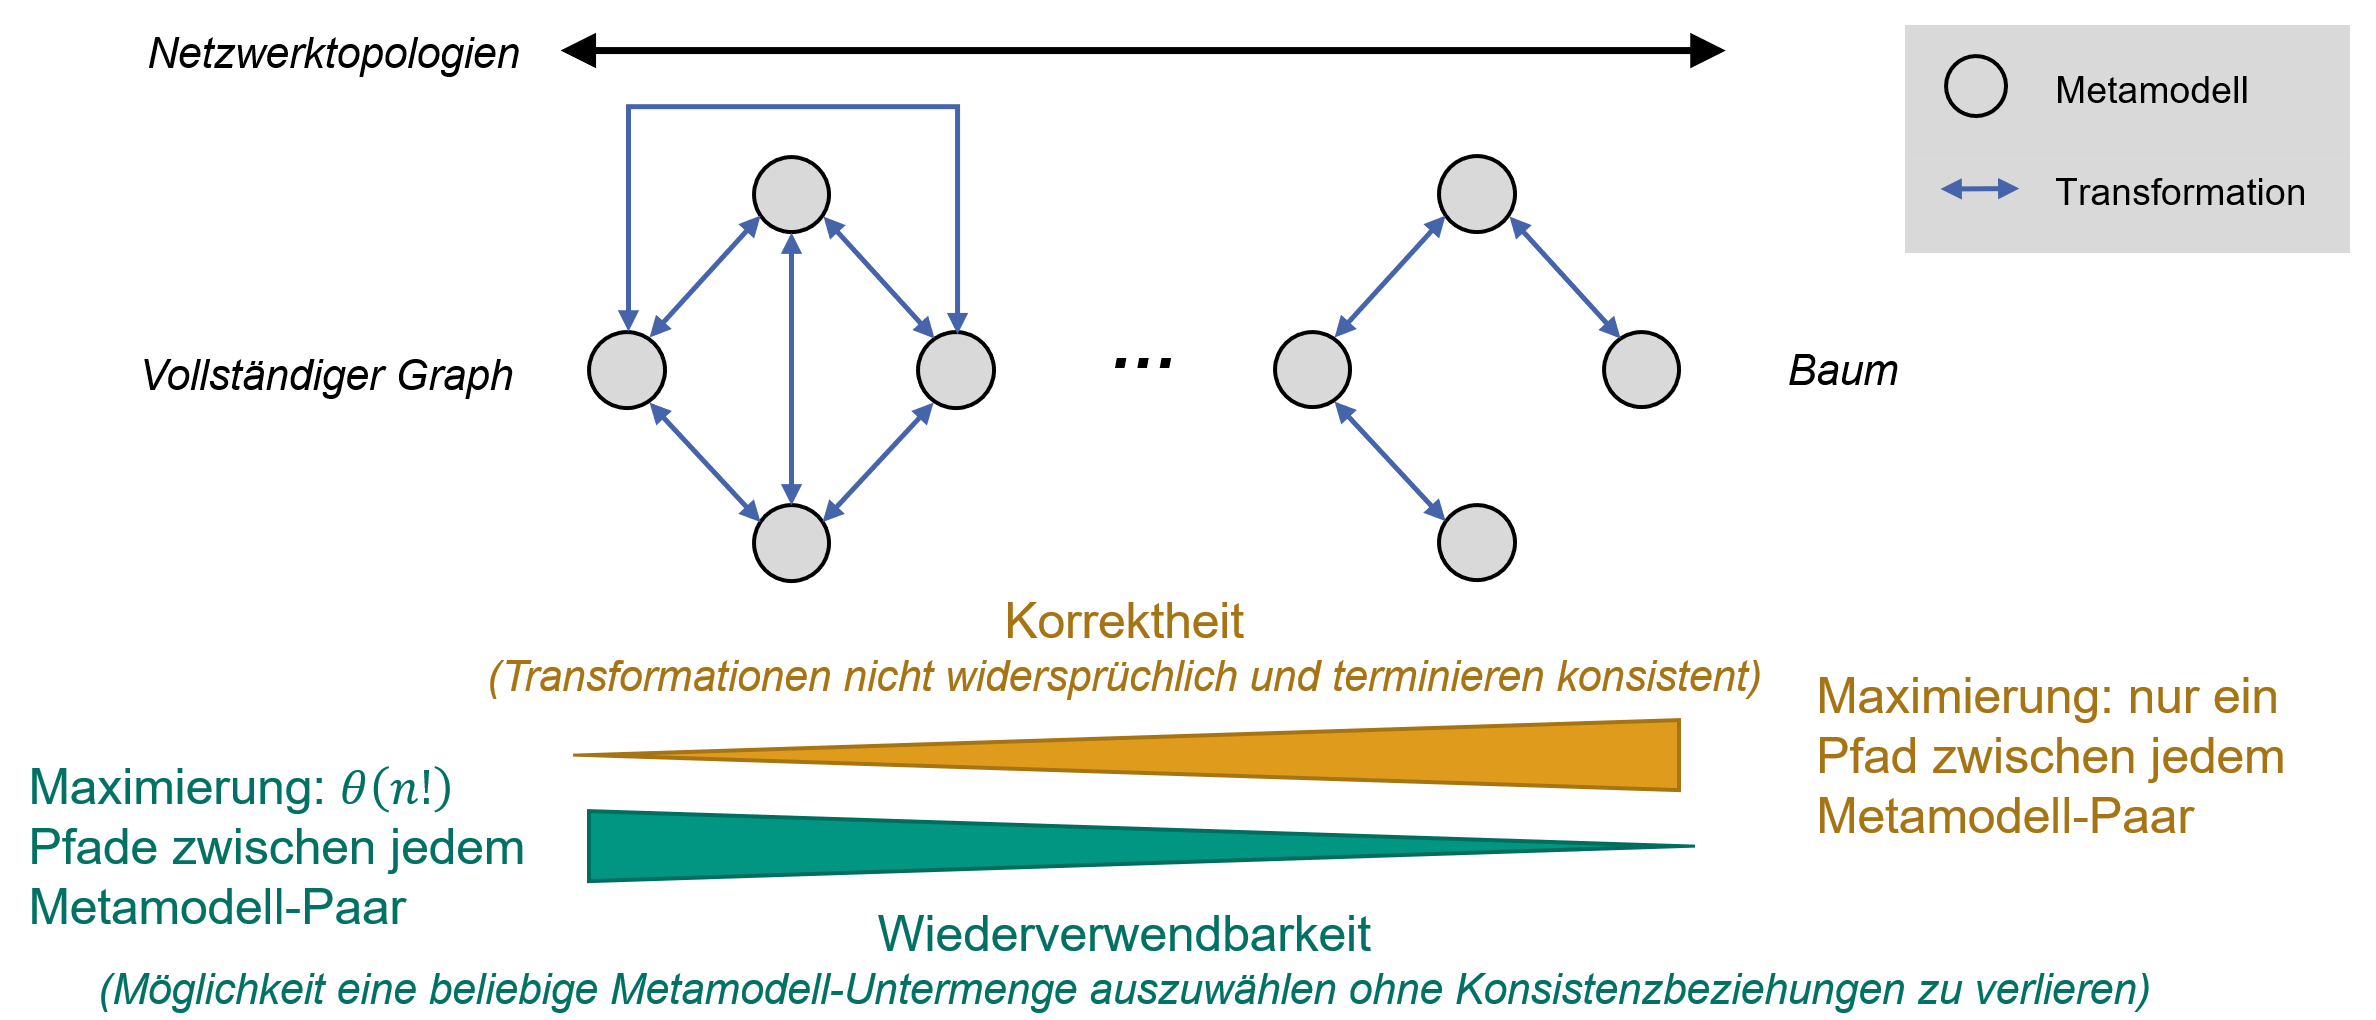
\includegraphics[width=\textwidth]{figures/quality/classification/tradeoff.png}
%     \caption[Trade-off between correctness and reusability]{Trade-off between quality properties at the example of correctness and reusability depending on the network topology.}
%     \label{fig:classification:tradeoff}
% \end{figure}

\mnote{Gradual improvement in actual networks}
An actual transformation network will usually neither induce a complete graph nor a tree, although we have already discussed that complete graphs are at least easier to achieve.
Thus, a network will not inherently optimize any of these properties but gradually optimize some of them, depending on the number of duplications of preservation for consistency relations within the transformations.
This leads to a trade-off between different properties depending on the achieved topology.
More duplications lead to higher completeness and reusability, whereas less duplications improve inherent correctness and also likely improve further discussed quality properties. %, such as modularity, analyzability, modifiability and testability.
%We depict this trade-off exemplarily in \autoref{fig:classification:tradeoff} for correctness and reusability as two of the essential properties inherently optimized by the extreme topologies.

\mnote{Benefit of trees}
Although trees are not easy to achieve in practice due to the missing ability of transformation networks with such a topology to express every possible consistency relation, their inherent correctness guarantee is still interesting, as we have seen how difficult correctness is to achieve in networks of arbitrary topology in the previous chapters.
In the following chapter, we thus identify and discuss how we can use this essential benefit of trees to construct networks that still provide a high level of completeness and reusability.

\mnote{Fine-grained topology notion}
In fact, we have up to now discussed the topology of transformation networks at the level of complete metamodels and transformations between them.
Transformations are, however, composed of rules that preserve consistency according to fine-grained consistency relations, such as the ones we have specified in \autoref{def:consistencyrelation}.
Thus, we can even generalize the insights regarding topologies from complete metamodels and transformations to metamodel elements and fine-grained consistency relations, which then mitigates some of the drawbacks regarding completeness of trees.
This conforms to the notion of \emph{non-interference} defined by \textcite{stevens2020BidirectionalTransformationLarge-SoSym}, which considers transformations to be non-interfering as long as they affect independent subsets of the metamodels and thus can be executed in any order.


% Modularity, independence, correctness and comprehensibility directly induced by specific topologies
% Universality not given for trees, has to be ensures for dense graphs (depends on orchestration strategy, see existing work)
% Trade-off between Modularity/Independence (inherent in dense graph) and Correctness/Comprehensibility (inherent in tree)

% Realizing consistency relations in transitive transformations can, for example, reduce comprehensibility, as a developer has to consider a set of transformations to understand a single consistency relation. 


% \begin{copiedFrom}{DocSym}

% %As discussed during the presentation of the challenges in the previous section, 
% We will focus on compatibility and modularity, as they are crucial for the applicability of transformations. %, whereas comprehensibility and development effort can be seen as usability problems. %, so we focus on those former two challenges.
% Defining binary transformations %to express consistency preservation 
% for a set of metamodels leads to a trade-off solution regarding those challenges, as they cannot be solved simultaneously.
% The intuitive way to define transformations %preservation of consistency relations is achieved by expressing each relation in a transformation.
% is to express each relation between two metamodels in one transformation, which leads to a dense graph of transformations. % between the metamodels.
% In the extreme case, if all pairs of metamodels have non-empty consistency relations, the graph is complete, as shown in \autoref{fig:classification:topologies:complete}.
% In that case, modularity is high because each metamodel can be excluded without any drawback, %, comprehensibility is rather high as each relation is expressed directly between the involved metamodels, %(although it may be additionally expressed transitively), 
% but relations are likely to be incompatible, as, in the worst case, each relation is specified over $(n-1)!$ transformation paths if $n$ metamodels are involved.
% While comprehensibility is high, as each relation is explicitly expressed, adding a metamodel requires to define up to $n-1$ transformations, implying high evolution effort.
% %Finally, this also implies a high development effort, as adding a metamodel requires to define transformations to all existing ones.

% Another extreme case is to have each consistency relation only defined over a single path in the transformations graph, which results in a tree of transformations, as shown in \autoref{fig:classification:topologies:tree}.
% In that case, compatibility of transformations is inherently given, as each relation is only defined once, but modularity is reduced, as only metamodels being leaves can be omitted.
% Comprehensibility is low, as each relation may be defined in a path of up to $n-1$ transformations, but evolvability is rather good, as each relation must only be defined once. %, but in a way such that the tree structure is maintained. %requires a critical investigation about how to express the consistency relations to maintain the tree structure.
% We summarize that impact of the topology in \autoref{tab:classification:topology_impact}.

% %In the following sections, we discuss our proposed solutions on how to deal with those trade-offs.
% \begin{table}
%     \centering
%     \begin{tabular} {L{8em} C{6em} C{5em}}
%         \toprule
%         \textbf{Challenge} & \textbf{Dense Graph} & \textbf{Tree}\\
%         \midrule
%     %    Uniqueness & - - & ++\\
%         Compatibility & - & ++\\
%         Modularity & ++ & -\\
%         Comprehensibility & + & -\\
%         Evolvability & - & +\\
%         \bottomrule
%     \end{tabular}
%     \caption{Challenge fulfillment by transformation topology}
%     \label{tab:classification:topology_impact}
%     \vspace{-1.5em}
% \end{table}

% A tree topology has the drawback that it is not always applicable.
% It requires that the transformation developers
% %\todoErik{whom?}
% find a subset of all consistency relations between the metamodels that induces a tree and whose transitive closure contains all other relations.
% %This is necessary, because the transitive relations in the tree must also cover the direct relations between the metamodels that are omitted.
% In general, such a subset cannot be found.
% Of three metamodels, there must always be one containing the overlapping information of the two others, as only then the transitive closure of two consistency relations subsumes the third. 
% In the example in \autoref{fig:classification:tree_generation}, it is necessary that two relations are contained in the transitive closure of the others to get a tree that covers all relations.
% %An example for such a relation is given in the graphic.

% \begin{figure}[b]
%     \centering
%     \newcommand{\mmdistance}{4em}

\begin{tikzpicture}[
    mm/.style={schematic metamodel},
]

% graph

\node[mm] (graph_top) {};
\node[mm, below=\mmdistance of graph_top.center, anchor=center] (graph_middle) {};
\node[mm, below left=0.5*\mmdistance and sqrt(3)/2*\mmdistance of graph_middle.center, anchor=center] (graph_bottomleft) {};
\node[mm, below right=0.5*\mmdistance and sqrt(3)/2*\mmdistance of graph_middle.center, anchor=center] (graph_bottomright) {};

\draw[consistency relation] (graph_top) -- node[left] {$R_2$} (graph_middle);
\draw[consistency relation] (graph_top) to[bend right=40] node[pos=0.3, above left] {$R_1$} (graph_bottomleft);
\draw[consistency relation] (graph_top) to[bend left=40] node[pos=0.3, above right] {$R_3$} (graph_bottomright);
\draw[consistency relation] (graph_middle) -- node[pos=0.4, above left] {$R_4$} (graph_bottomleft);
\draw[consistency relation] (graph_middle) -- node[pos=0.4, above right] {$R_5$} (graph_bottomright);

% tree

\node[mm, right=4*\mmdistance of graph_top] (tree_top) {};
\node[mm, below=\mmdistance of tree_top.center, anchor=center] (tree_middle) {};
\node[mm, below left=0.5*\mmdistance and sqrt(3)/2*\mmdistance of tree_middle.center, anchor=center] (tree_bottomleft) {};
\node[mm, below right=0.5*\mmdistance and sqrt(3)/2*\mmdistance of tree_middle.center, anchor=center] (tree_bottomright) {};

\draw[consistency relation] (tree_top) -- node[left] {$R_2$} (tree_middle);
\draw[consistency relation] (tree_middle) -- node[pos=0.4, above left] {$R_4$} (tree_bottomleft);
\draw[consistency relation] (tree_middle) -- node[pos=0.4, above right] {$R_5$} (tree_bottomright);


\draw[latex-latex] ([yshift=0.2*\mmdistance, xshift=1.1*\mmdistance]graph_middle.east) -- 
    node[above] {$R_2 \concat R_4 \subseteq R_1$} 
    node[below] {$R_2 \concat R_5 \subseteq R_3$}
    ([yshift=0.2*\mmdistance, xshift=-1*\mmdistance]tree_middle.west);

\end{tikzpicture}
%     \caption{Reducing a consistency relation graph to a tree}
%     \label{fig:classification:tree_generation}
% \end{figure}

% In practice, the used topology will potentially be a mixture between those extremes.
% The natural way to foster the independent development of transformations %to specify consistency preservation 
% would be to define one transformation for each consistency relation, resulting in a dense graph with a high potential for incompatible transformations.
% To deal with that, mechanisms that analyze compatibility between transformations could be researched.
% Nevertheless, high expressiveness of transformation languages allows only conservative approximations. % without reducing the expressiveness of transformation languages, this easily leads to problems similar to those in static code analysis, which rely on approximations, due to the Halting problem.
% In our thesis, we will therefore investigate approaches that result in tree-like specifications that directly imply compatibility between the transformations, but with increased \emph{applicability} and \emph{modularity}. %of  try to achieve a tree of transformations, as this directly implies consistency between the transformations, but with increased modularity and with applicability.

% \end{copiedFrom} % DocSym


\section{Summary}

In this chapter, we have discussed which software quality properties, as defined in an ISO standard~\cite{iso25010}, are relevant for developers of transformation networks.
In addition, we have identified two extremes of transformation network topologies and discussed their impacts on quality properties.
From this discussion, we were are able to derive necessary trade-offs between the properties induced by the topology of the network.
We conclude this chapter with the following central insight.

\begin{insight}
    In addition to functional correctness of transformation networks, further quality properties can be relevant for developers and user of such networks.
    For developers of transformations networks, in particular functional completeness, i.e., the ability to apply transformation networks to any situation in which consistency between models needs to be preserved, and different aspects of maintainability, such as modularity, reusability, analyzability, modifiability and testability, are important.
    Transformation networks induce a graph of metamodels and transformations between them that can, at one extreme, be a complete graph, in which each pair of metamodels is directly related by a transformation, and, at the other extreme, be a tree, in which each pair of metamodels is only related by one path of transformations.
    While networks inducing a complete graph inherently optimize completeness and reusability, those inducing a tree inherently optimize correctness.
    Although trees are particularly restrictive regarding completeness and in practice networks inducing a tree are thus hard to achieve, their inherent correctness guarantee makes them still interesting, as they avoid multiple challenges to achieve correctness.
\end{insight}
